En la figura \ref{fig:diagrama_bloques}, se muestra el diagrama de bloques general desarrollado en \textit{LabVIEW}.

\begin{figure}[H]
    \centering
    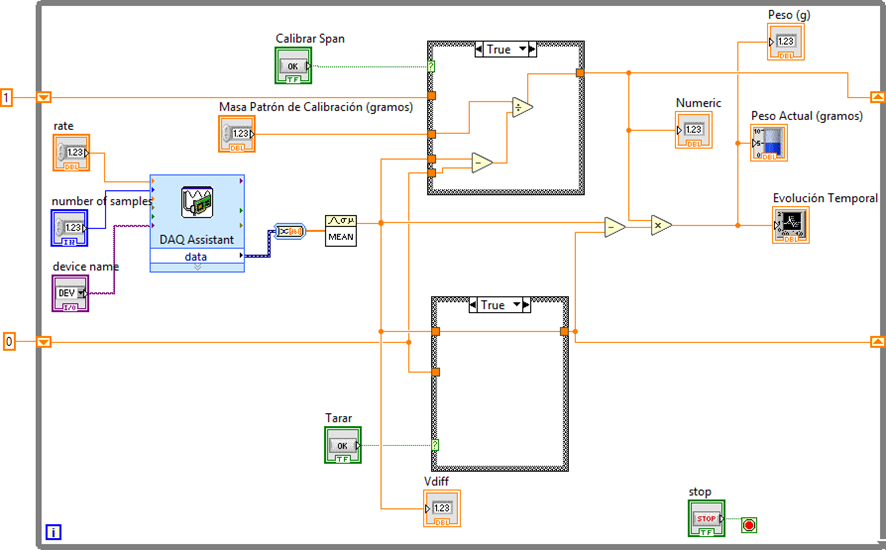
\includegraphics[width=1\linewidth]{figs/diagrama_bloques_LABVIEW.png}
    \caption{Diagrama de Bloques general en \textit{LabVIEW}.}
    \label{fig:diagrama_bloques}
\end{figure}

La ejecución del programa está encapsulada dentro de un bucle \textit{While}, lo que permite la iteración ininterrumpida del proceso de lectura, cálculo y visualización hasta que el operador detenga el sistema de manera manual mediante el control de parada incorporado en la interfaz.


\subsection{Adquisición y Acondicionamiento de la Señal}

Se utilizó el bloque \textit{DAQ Assistant}, el cual está configurado para interrogar al hardware físico. Se seleccionó un terminal de entrada en modo diferencial frente a la configuración RSE (Referenciado a Masa), tal como se ilustra en la figura \ref{fig:diferencial}. Esta decisión de diseño es imperativa para preservar el factor de rechazo al modo común (CMRR) de la etapa de acondicionamiento analógico previa, mitigando el ruido eléctrico en modo común inducido en las líneas de transmisión de la señal de bajo nivel proveniente de la célula de carga.

\begin{figure}[H]
    \centering
    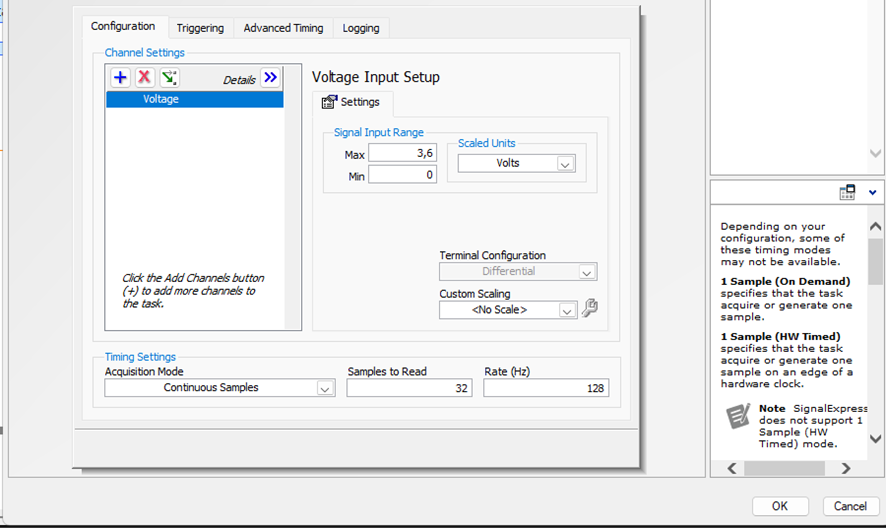
\includegraphics[width=0.75\linewidth]{figs/diferencial.png}
    \caption{Configuración en Modo diferencial en el módulo \textit{DAQ Assistant}.}
    \label{fig:diferencial}
\end{figure}

Este bloque adquiere la señal de tensión analógica, parametrizando un rango de tensión de $\pm3.6$ V] para maximizar la resolución del convertidor. La lectura de la información se realiza en paquetes definidos por una frecuencia de muestreo (\textit{Rate}) de 128 Hz y un número de muestras (\textit{Samples to Read}) establecido en exactamente 32 muestras.

Esta ventana de promediado estadístico por software se justifica como el punto de operación óptimo del instrumento virtual: un número inferior de muestras resultaría en un filtrado insuficiente del ruido térmico y de cuantización, provocando inestabilidad en el dígito menos significativo de la lectura física; por el contrario, una ventana mayor introduciría una latencia considerable en el bucle, degradando el tiempo de respuesta dinámico de la báscula frente a variaciones súbitas de carga. Los datos dinámicos obtenidos en esta ventana pasan de forma directa por un bloque estadístico de media aritmética (\textit{Mean}), entregando un único valor de tensión estabilizado para las etapas posteriores de procesamiento matemático.

\subsection{Arquitectura del VI y Gestión de Memoria Dinámica}

Para mantener las constantes de calibración actualizadas y disponibles ciclo tras ciclo, el diagrama de bloques emplea dos registros de desplazamiento (\textit{Shift Registers}) ubicados en los bordes laterales del bucle \textit{While} principal:

\begin{itemize}
    \item \textbf{Registro Superior (Factor de \textit{Span}):} Inicializado con una constante de valor 1, almacena el multiplicador dinámico que convierte la magnitud eléctrica neta a unidades físicas de masa (gramos).
    \item \textbf{Registro Inferior (Tensión de Tara):} Inicializado en 0 V, retiene el valor de la tensión residual medida sin carga, el cual se corresponde con el cero del sistema.
\end{itemize}

En la figura \ref{fig:estructuras_case} se detalla la lógica interna de almacenamiento según los estados de control del operador.

\begin{figure}[H]
    \centering
    \begin{subfigure}[b]{0.48\textwidth}
        \centering
        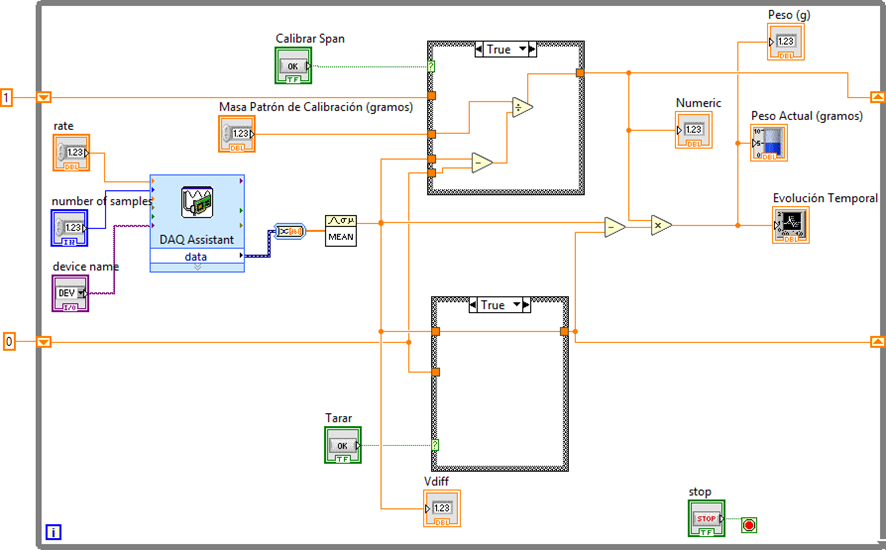
\includegraphics[width=\textwidth]{figs/diagrama_bloques_LABVIEW.png}
        \caption{Diagrama de bloques (Caso \textit{True}).}
        \label{fig:labview_caso_true}
    \end{subfigure}
    \hfill
    \begin{subfigure}[b]{0.48\textwidth}
        \centering
        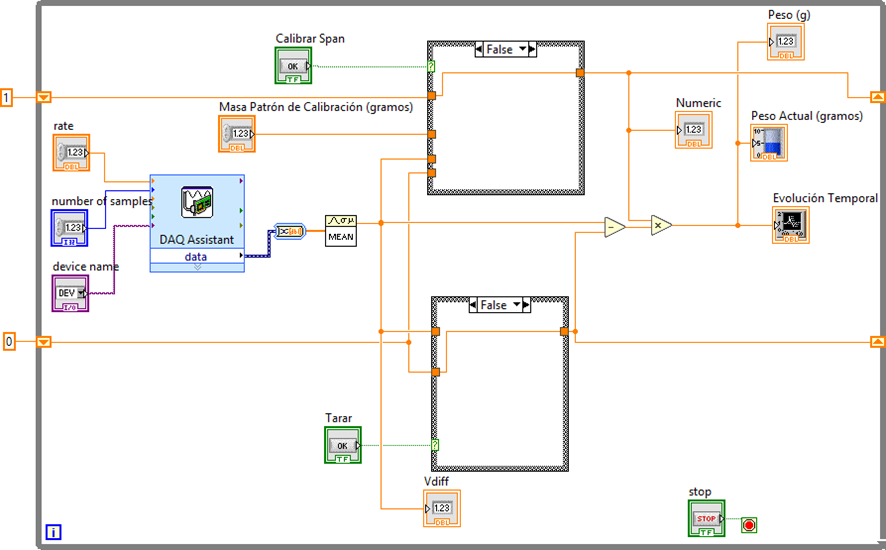
\includegraphics[width=\textwidth]{figs/labview_caso_false.png}
        \caption{Diagrama de bloques (Caso \textit{False}).}
        \label{fig:labview_caso_false}
    \end{subfigure}
    \caption{Comportamiento de la arquitectura interna del VI según los eventos de control.}
    \label{fig:estructuras_case}
\end{figure}

\subsection{Lógica Matemática y Rutinas Condicionales de Calibración}

El software cuenta con un algoritmo de calibración lineal de dos puntos gestionado por estructuras \textit{Case}. Estas rutinas son accionadas a voluntad por el usuario a través del Panel Frontal:

\begin{itemize}
    \item \textbf{Establecimiento del Cero (Tara):} Controlado por la estructura inferior (ver figura \ref{fig:establecer_cero_labview}). Al recibir un comando lógico verdadero (\textit{True}) tras pulsar el botón de tara, el programa captura la tensión promedio instantánea de ese ciclo exacto y la sobrescribe en el \textit{Shift Register} inferior. En su estado inactivo (\textit{False}), el último valor registrado simplemente atraviesa la estructura para mantenerse intacto en la memoria dinámica.
    \item \textbf{Calibración del \textit{Span}:} Controlada por la estructura superior (ver figura \ref{fig:establecer_span}). Al introducir el valor de la masa patrón en la interfaz y activar esta rutina, el programa recalcula la pendiente de medición. Obtiene la tensión neta bajo carga y ejecuta la siguiente relación matemática:

          $$Factor=\frac{\text{Masa}_{\text{referencia}}}{V_{leido}-V_{tara}}$$

          El resultado numérico de esta operación sobrescribe el registro de desplazamiento superior, actualizando la sensibilidad global del instrumento de manera instantánea.
\end{itemize}

\begin{figure}[H]
    \centering
    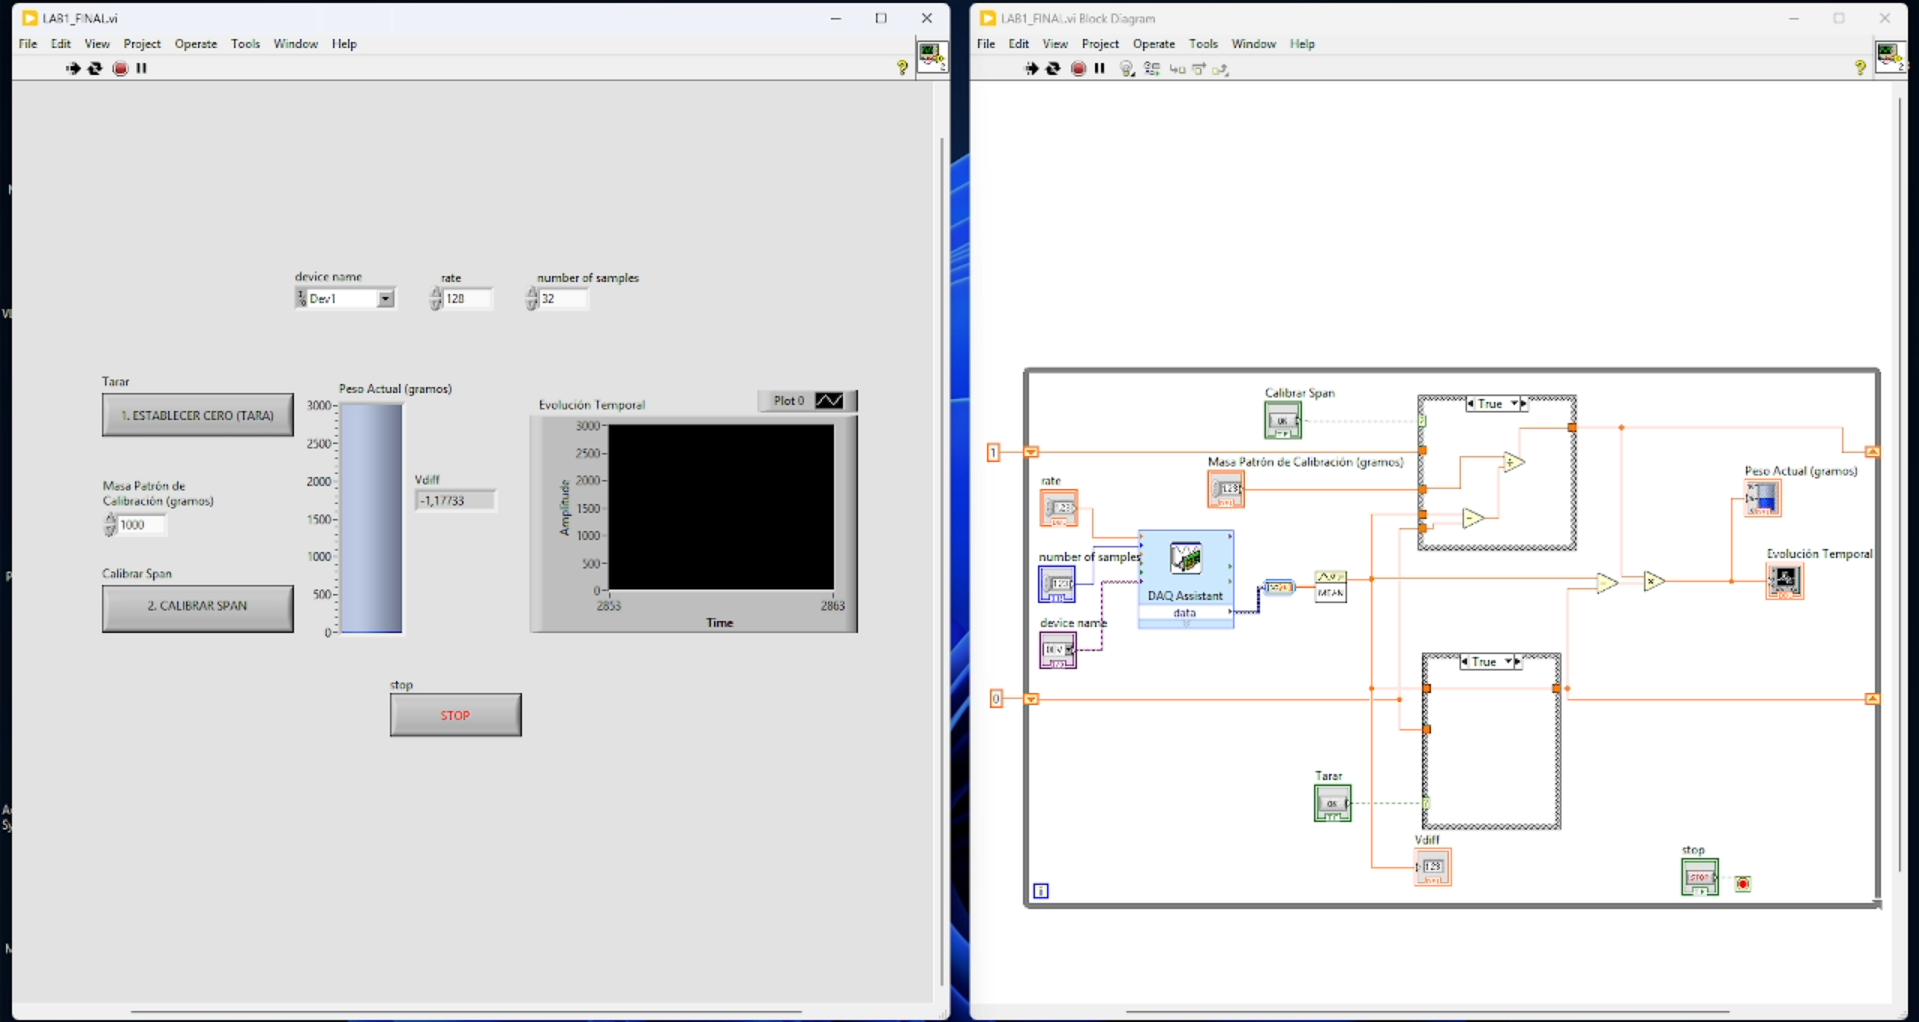
\includegraphics[width=1\linewidth]{figs/establecer_cero_labview.png}
    \caption{Diagrama de bloques ante la activación del evento de Establecer Cero.}
    \label{fig:establecer_cero_labview}
\end{figure}

\begin{figure}[H]
    \centering
    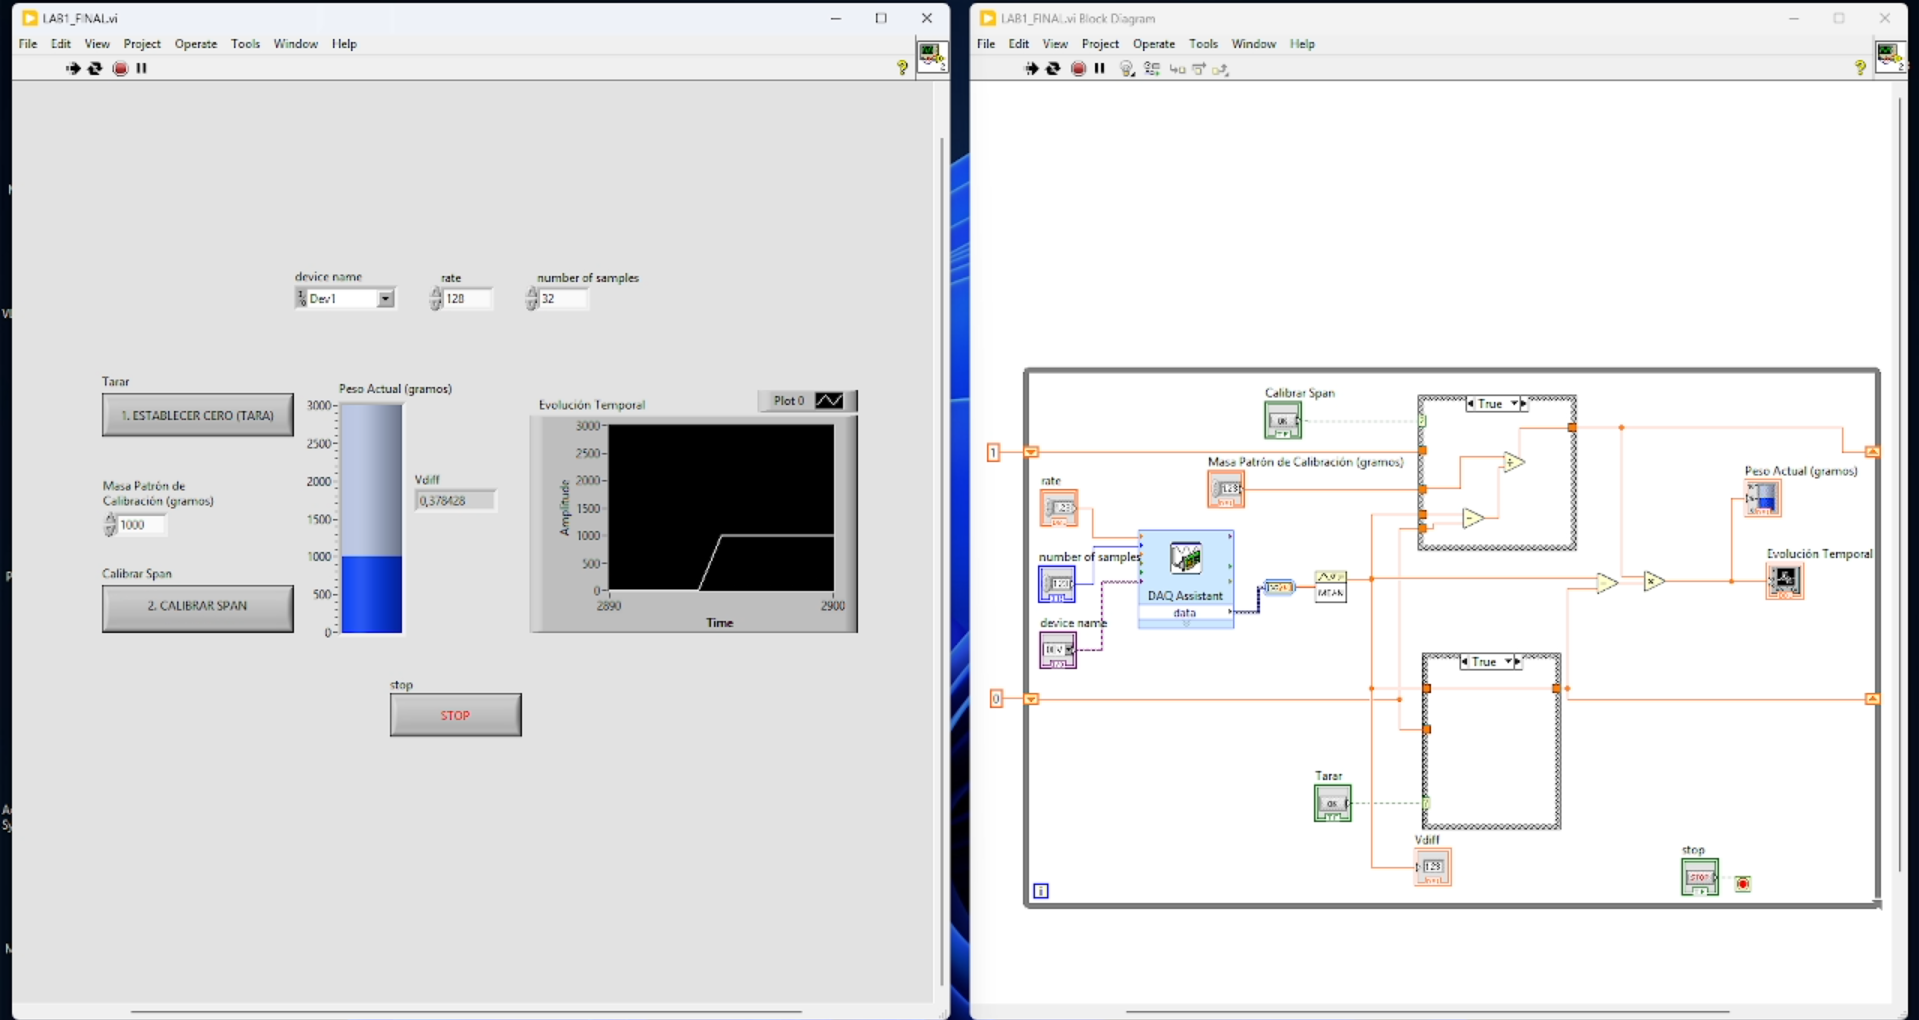
\includegraphics[width=1\linewidth]{figs/establecer_span.png}
    \caption{Diagrama de bloques ante la activación del ajuste de \textit{Span} utilizando la masa patrón de 1.000 kg.}
    \label{fig:establecer_span}
\end{figure}

\subsection{Procesamiento Final, Monitorización e Interfaz de Usuario}

De forma paralela a las lógicas condicionales, el diagrama ejecuta en cada iteración el cálculo lineal definitivo para obtener la masa real. Utilizando nodos aritméticos elementales, se aplica la ecuación de la recta basada en las señales en tiempo real y las constantes retenidas en la memoria dinámica:

$$Peso=(V_{leido}-V_{tara}) \times Factor$$

El resultado numérico representa la magnitud calibrada final. A nivel de Panel Frontal, la interfaz ha sido diseñada bajo criterios ergonómicos, priorizando la legibilidad metrológica de los indicadores. La magnitud calculada alimenta simultáneamente tres elementos gráficos visualmente jerarquizados: un indicador numérico de gran tamaño para la lectura directa rápida, un indicador de barra vertical para evaluar el rango dinámico consumido respecto al fondo de escala (\textit{FSO}), y un gráfico de tipo \textit{Waveform Chart}. Este último elemento gráfico es vital desde la perspectiva metrológica, pues permite al operador monitorizar visualmente la estabilidad temporal del puente, evaluar el tiempo de asentamiento de la señal tras depositar una masa y verificar la correcta mitigación del ruido analógico por el software.

En las figuras \ref{fig:pesajecero} y \ref{fig:pesajedeprueba} se muestra el comportamiento operativo de la interfaz en sus dos estados fundamentales de carga.

\begin{figure}[H]
    \centering
    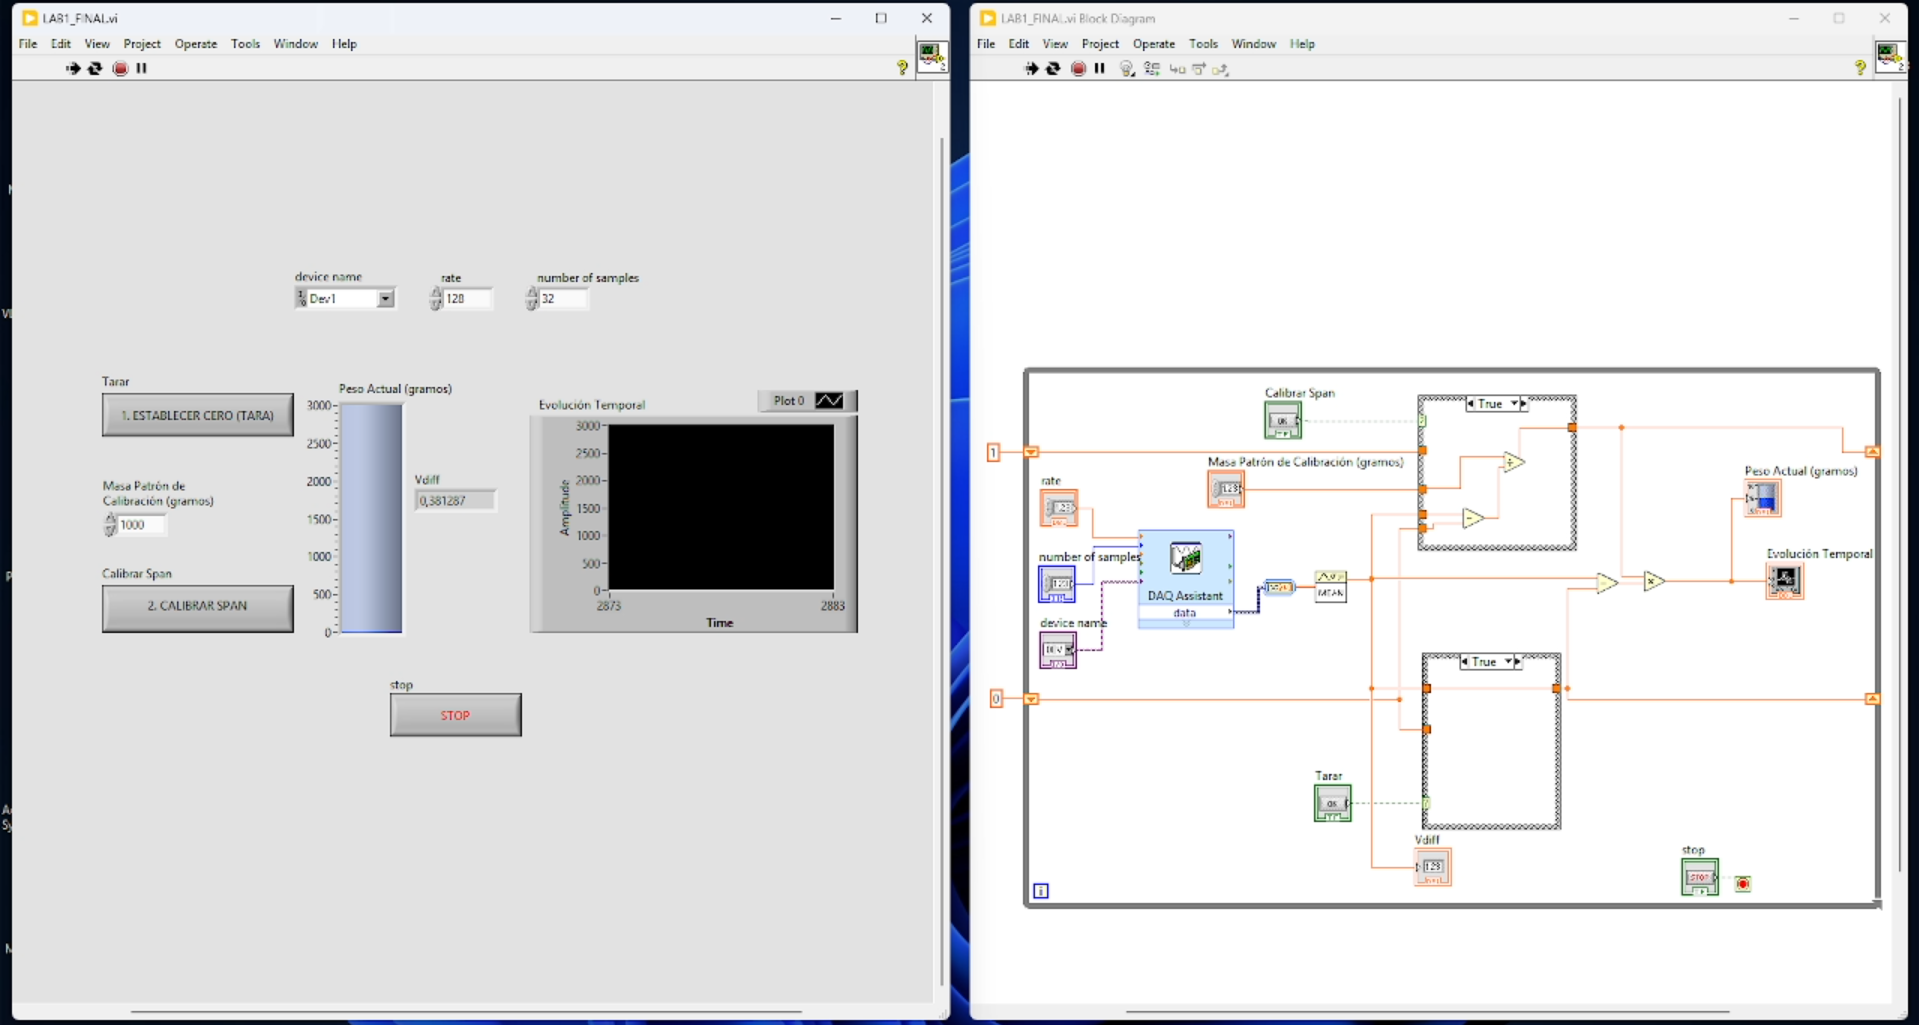
\includegraphics[width=1\linewidth]{figs/pesajecero.png}
    \caption{Interfaz del Panel Frontal en estado de reposo (Fijación del cero metrológico).}
    \label{fig:pesajecero}
\end{figure}

\begin{figure}[H]
    \centering
    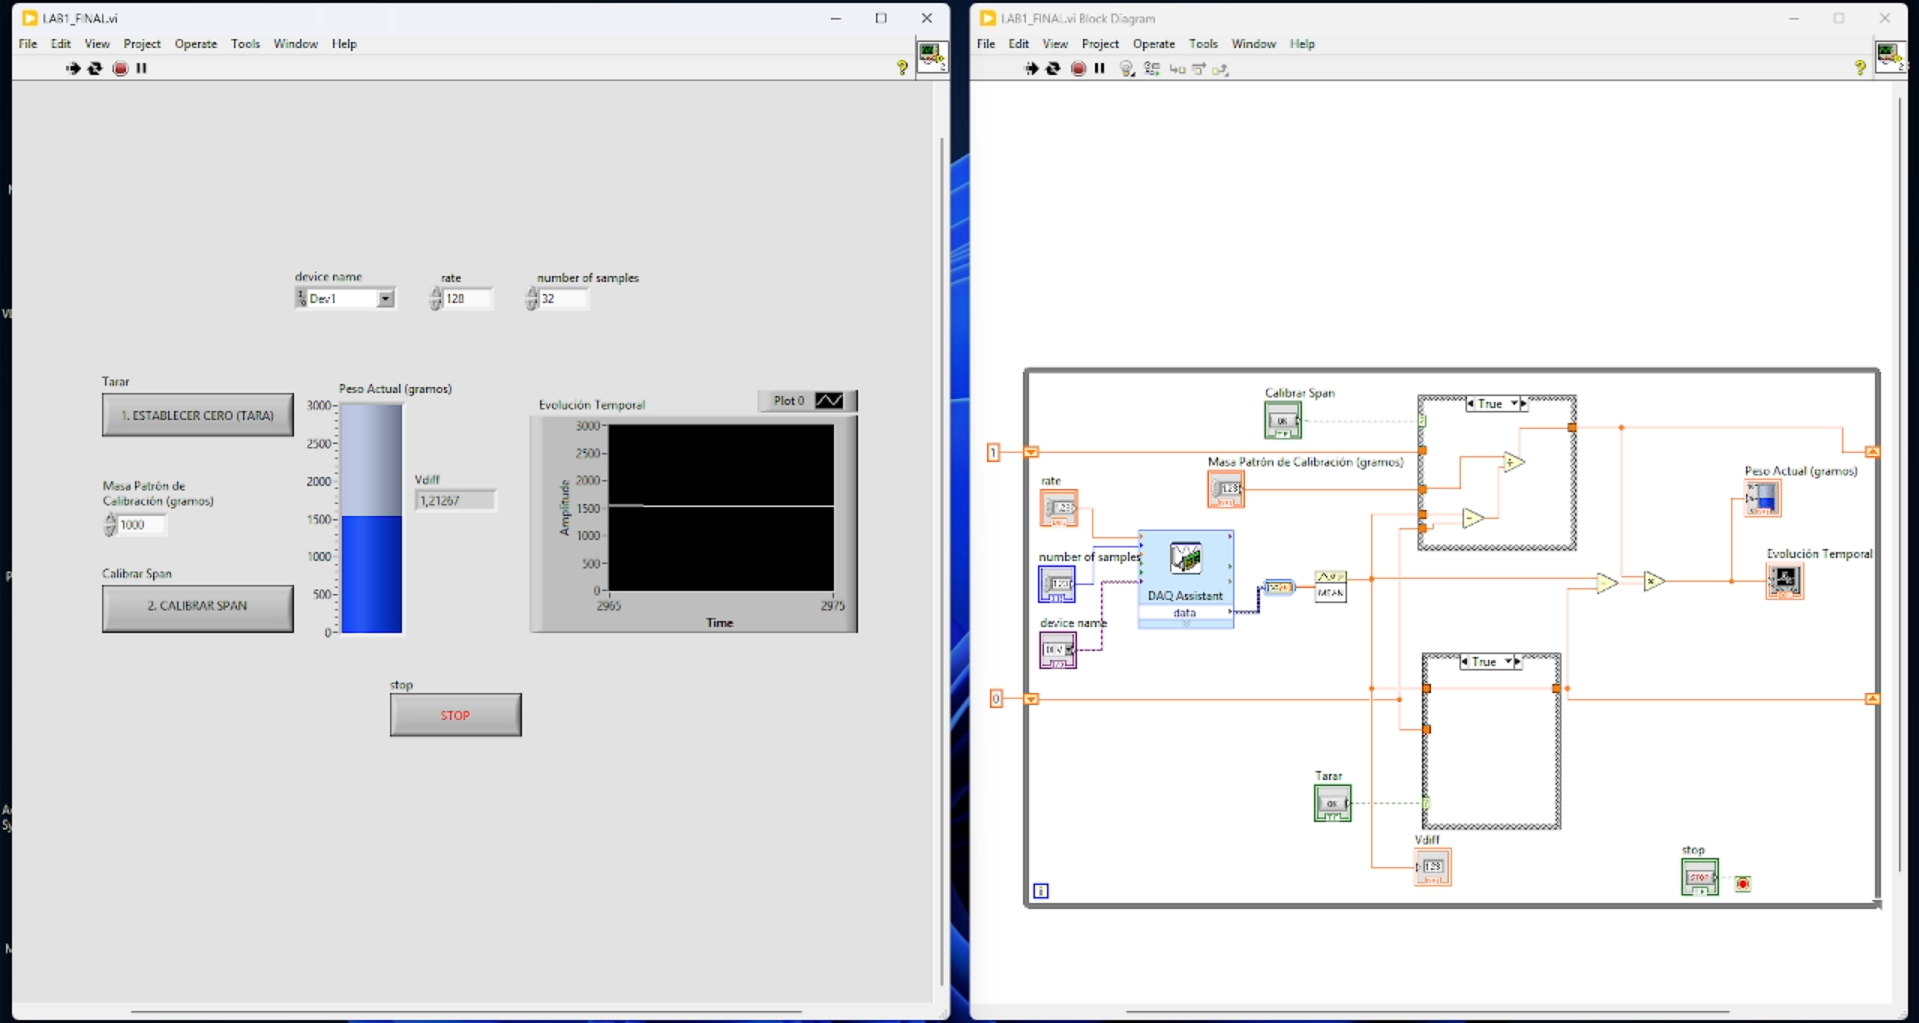
\includegraphics[width=1\linewidth]{figs/pesajedeprueba.png}
    \caption{Validación experimental del sistema mediante el pesaje de una masa de prueba de 1.5 kg.}
    \label{fig:pesajedeprueba}
\end{figure}